\documentclass[c]{beamer}
\usepackage{org-preamble}
\usepackage[cpp_teaching]{slide-style}
\usepackage{minted}
\newcommand{\inline}[1]{\mintinline[breaklines]{c++}{#1}}
\usetheme{default}
\usepackage{tikz}
\AtBeginSection[]{
  \begin{frame}
  \centering
  \begin{beamercolorbox}[sep=8pt,center,shadow=true,rounded=true]{title}
    \usebeamerfont{title}\insertsectionhead\par%
  \end{beamercolorbox}
  \end{frame}
}

\title{Encapsulation des données, constructeurs, destructeurs, copie}
\subtitle{Ou comment faire les choses proprement.}

\begin{document}

\maketitle

\section{Constructeurs et destructeurs}


\begin{frame}[fragile]{Constructeur de classe}
\begin{itemize}
\item Le constructeur et le destructeur sont deux \structure{méthodes \emph{i.e.} fonctions
membres} particulières

\begin{itemize}
\item le constructeur est appelé à la création d'un objet,
\item le destructeur est appelé à la destruction d'un objet.
\end{itemize}

\item constructeur \(\equiv\) \structure{initialisation des membres}
\begin{itemize}
\item allocation dynamique de mémoire,
\item ouverture de connexion, de fichier, de fenêtre...
\end{itemize}

\item destructeur \(\equiv\) \structure{ultimes opérations}
\begin{itemize}
\item désallocation de la mémoire précédemment allouée
\item fermeture des ressources, déconnexion...
\end{itemize}

\end{itemize}
\end{frame}

\begin{frame}[fragile]{Constructeur de classe}
\begin{itemize}
\item Le constructeur est une méthode à part entière (d'où la possibilité de la
  surdéfinir) néanmoins
  
\begin{itemize}
\item le constructeur doit porter \structure{le même nom} que la classe,

\item le constructeur ne doit avoir \structure{aucun type} de retour (pas même void).
\end{itemize}
\end{itemize}
\end{frame}

\begin{frame}[fragile]{Déclaration de constructeurs}
\begin{minted}[fontsize=\footnotesize,samepage,mathescape,xrightmargin=0.5cm,xleftmargin=0.5cm]{c++}
class Matrice {
public:
  // Constructeur sans arguments (par défaut) : matrice vide
  Matrice();

  // Surdéfinition de constructeur : matrice de cols ⨉ rows
  Matrice(unsigned int cols, unsigned int rows, double valdef=0.);

private:
  double* data;
  unsigned int cols, rows;
};
\end{minted}
\end{frame}

%-----------

\begin{frame}[fragile]{Définition de constructeurs}

Dans \texttt{matrice.cpp} :

\begin{minted}[fontsize=\footnotesize,samepage,mathescape,xrightmargin=0.5cm,xleftmargin=0.5cm]{c++}
#include "matrice.h"

Matrice::Matrice(unsigned int cols_, unsigned int rows_, double valdef) {
  cols = cols_;
  rows = rows_;
  data = new double[cols*rows];
  for (unsigned int k = 0; k < cols*rows; k++)
    data[k] = valdef;
  std::cout << "Matrice " << cols << "x" << rows << " crée @" << data << ".\n";
}

Matrice::Matrice() : Matrice(0,0) {}
\end{minted}

\vspace{1em}
Schématiquement, le compilateur va faire :
\begin{minted}[fontsize=\footnotesize,samepage,mathescape,xrightmargin=0.5cm,xleftmargin=0.5cm]{c++}
unsigned int cols;  // allocations
...
cols = cols_;  // initialisation
...
\end{minted}

\end{frame}

%-----------

\begin{frame}[fragile]{Définition de constructeurs avec \textit{initializer list}}

Dans \texttt{matrice.cpp} :

\begin{minted}[fontsize=\footnotesize,samepage,mathescape,xrightmargin=0.5cm,xleftmargin=0.5cm]{c++}
#include "matrice.h"

Matrice::Matrice(unsigned int cols_, unsigned int rows_, double valdef) 
  : cols(cols_), rows(rows_), data(nullptr)
{
  data = new double[cols*rows];
  for (unsigned int k = 0; k < cols*rows; k++)
    data[k] = valdef;
  std::cout << "Matrice " << cols << "x" << rows << " crée @" << data << ".\n";
}

Matrice::Matrice() : Matrice(0,0) {}
\end{minted}

\vspace{1em}
Schématiquement, le compilateur va faire :
\begin{minted}[fontsize=\footnotesize,samepage,mathescape,xrightmargin=0.5cm,xleftmargin=0.5cm]{c++}
unsigned int cols = cols_;
// allocation et initialisation au même moment
// (nécessaire quand le membre n'a pas de constructeur par défaut)
...
\end{minted}

\end{frame}

%-----------

\begin{frame}[fragile]{Utilisation}
\begin{minted}[fontsize=\footnotesize,samepage,mathescape,xrightmargin=0.5cm,xleftmargin=0.5cm]{c++}
#include "matrice.h"

void main () {

  Matrice matrice_vide;  // appel du constructeur par défaut

  Matrice matrice_pas_vide (3, 5, 1.42);
  // ou
  Matrice matrice_pas_vide = Matrice(3, 5, 1.42);

}
\end{minted}
\end{frame}

%-----------

\begin{frame}[fragile]{Destructeur de classe}
\begin{itemize}
\item Le destructeur est également une méthode, néanmoins

\begin{itemize}
\item le destructeur doit porter \structure{le même nom} que la classe \structure{préfixé du signe \texttt{\textasciitilde{}}},

\item le destructeur \structure{ne possède pas d'argument}; il n'est donc pas possible de surdéfinir cette méthode\footnote{logique, il ne peux n'y avoir qu'une seule façon de détruire un objet}.
\end{itemize}

\item Lors d'allocation dynamique de mémoire, la présence d'un destructeur est obligatoire
\end{itemize}
\end{frame}

%-----------

\begin{frame}[fragile]{Déclaration d'un destructeur}
\begin{minted}[fontsize=\footnotesize,samepage,mathescape,xrightmargin=0.5cm,xleftmargin=0.5cm]{c++}
class Matrice {
public:
  // Constructeurs
  Matrice();
  Matrice(unsigned int cols, unsigned int rows, double valdef=0.);

  // Destructeur
  ~Matrice();

  double* data;
  unsigned int cols, rows;
};
\end{minted}

Dans \texttt{matrice.cpp} :

\begin{minted}[fontsize=\footnotesize,samepage,mathescape,xrightmargin=0.5cm,xleftmargin=0.5cm]{c++}
Matrice::~Matrice() {
  if (data != nullptr)
    delete[] data;
  std::cout << "Matrice @" << data << " détruite.\n";
  data = nullptr;
}
\end{minted}

\end{frame}

%-----------

\begin{frame}[fragile]{Utilisation}
\begin{minted}[fontsize=\footnotesize,samepage,mathescape,xrightmargin=0.5cm,xleftmargin=0.5cm]{c++}
#include "Matrice.h"

void main () {

  cout << "Début\n";

  if (true) {
    Matrice matrice_pas_vide (3, 5, 1.);
    cout << "Milieu\n";
  }

  cout << "Fin\n";
}
\end{minted}
\pause
\begin{verbatim}
Début
Matrice 3x5 crée @0x56078abcc330.
Milieu
Matrice @0x56078abcc330 détruite.
Fin
\end{verbatim}

\end{frame}

%-----------------------------------------------------------------------------

\begin{frame}[fragile]{Cas particulier du constructeur par copie}

Il existe des situations autres que la déclaration d'objet où un constructeur est nécessaire,

\begin{itemize}[<+->]
\item lorsqu'un objet est passé par valeur en argument d'une fonction : \\ \inline{int rang (Matrice mat);}
\item lorsqu'un objet est renvoyé par valeur comme résultat d'une fonction : \\ \inline{Matrice matrice_alea ();}
\item lors de l'initialisation d'un objet par copie d'un objet du même type : \\ \inline{Matrice mat2 = mat1;}
\end{itemize}

\vspace{1em}
\onslide<+->{Par défaut, le compilateur génère un constructeur par copie trivial : les attributs sont simplement copiés}

\end{frame}

%-----------------------------------------------------------------------------


\begin{frame}[fragile]{Ça va mal se passer...}

\begin{minted}[fontsize=\footnotesize,samepage,mathescape,xrightmargin=0.5cm,xleftmargin=0.5cm]{c++}
{
  Matrice mat1 (3, 5)

  cout << "Avant\n";
  {
    Matrice mat2 = mat1;
    // modification de mat2...
  }
  cout << "Après\n";

  // utilisation de mat1...
}
\end{minted}

\pause

\begin{verbatim}
Matrice 3x5 crée @0x56078abcc330.
Avant
Matrice @0x56078abcc330 détruite.
Après
Matrice @0x56078abcc330 détruite.
\end{verbatim}

\end{frame}

%---------------------------------

\begin{frame}[fragile]{Ça va mal se passer...}
\begin{tikzpicture}[remember picture, overlay]
\node[] at (current page.center) 
{
    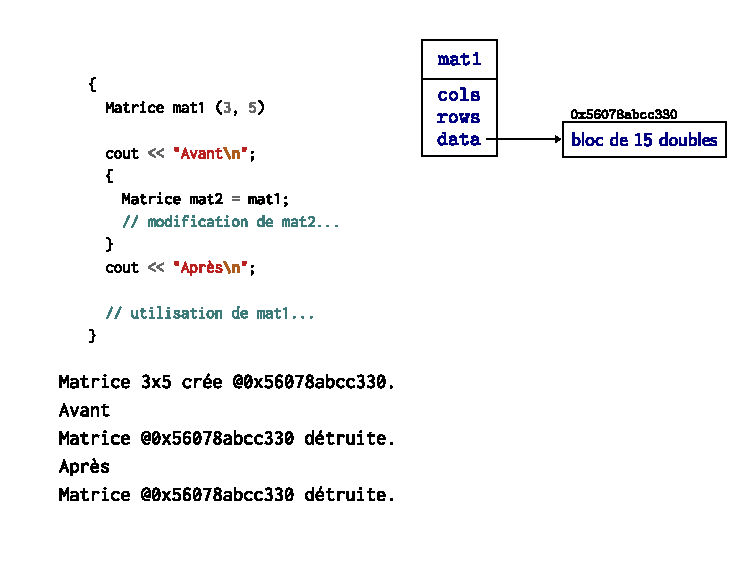
\includegraphics[scale=1]{copiefail1.pdf}
};
\end{tikzpicture}
\end{frame}

\begin{frame}[fragile]{Ça va mal se passer...}
\begin{tikzpicture}[remember picture, overlay]
\node[] at (current page.center) 
{
    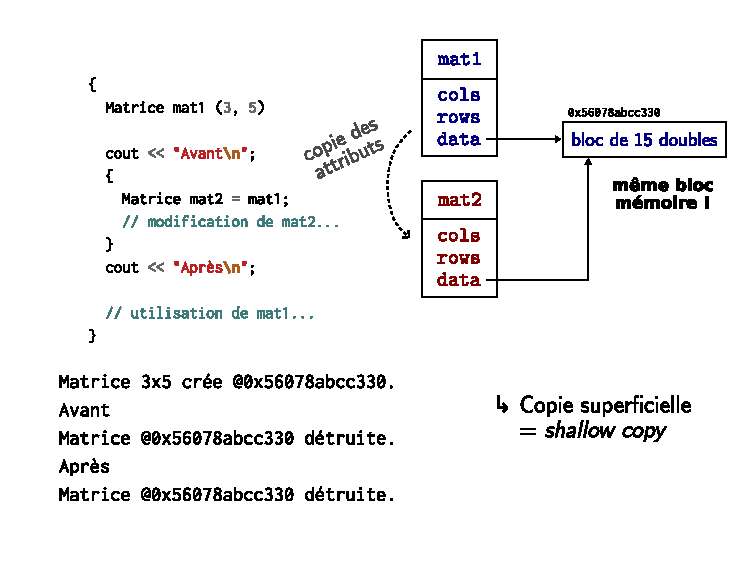
\includegraphics[scale=1]{copiefail2.pdf}
};
\end{tikzpicture}
\end{frame}

\begin{frame}[fragile]{Ça se passe mal}
\begin{tikzpicture}[remember picture, overlay]
\node[] at (current page.center) 
{
    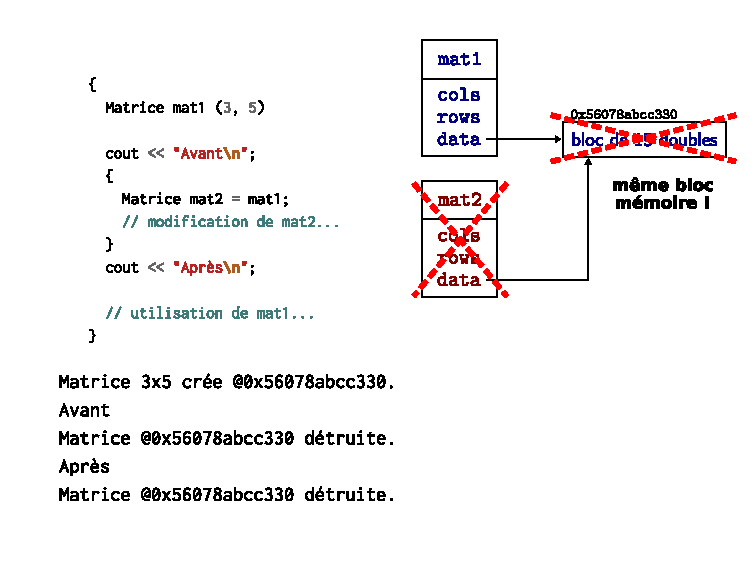
\includegraphics[scale=1]{copiefail3.pdf}
};
\end{tikzpicture}
\end{frame}

\begin{frame}[fragile]{Ça se passe mal}
\begin{tikzpicture}[remember picture, overlay]
\node[] at (current page.center) 
{
    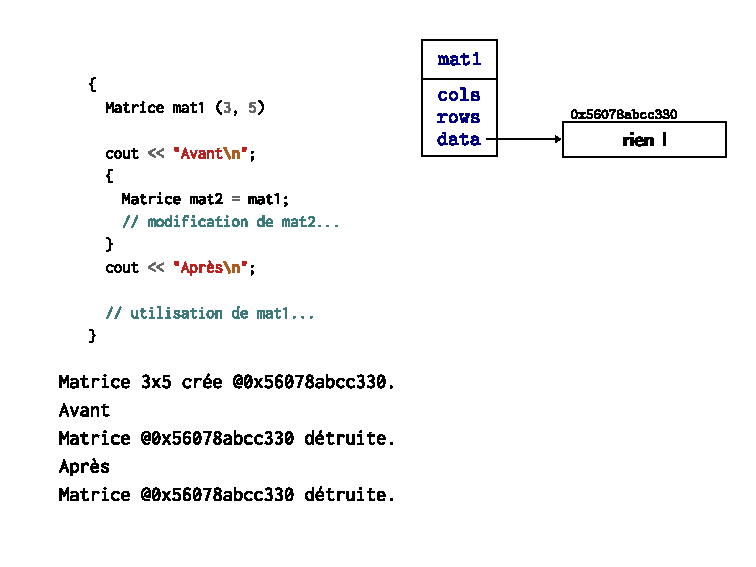
\includegraphics[scale=1]{copiefail4.pdf}
};
\end{tikzpicture}
\end{frame}

\begin{frame}[fragile]{Ce que l'on veut...}
\begin{tikzpicture}[remember picture, overlay]
\node[] at (current page.center) 
{
    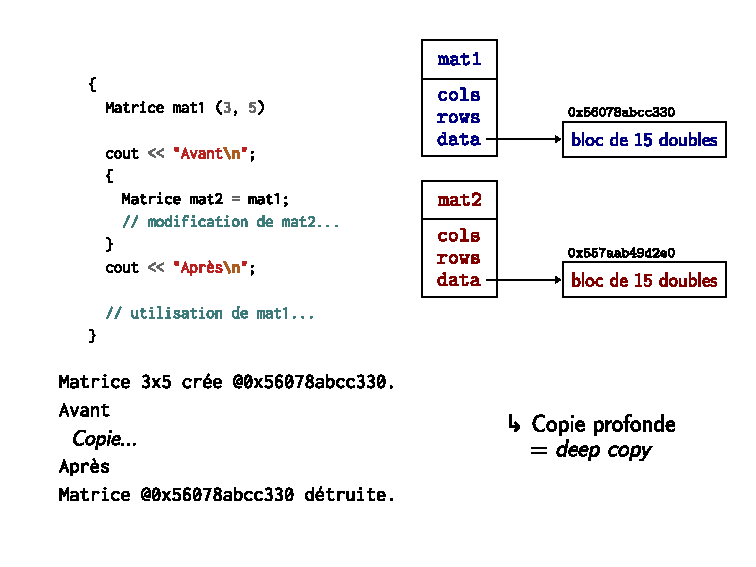
\includegraphics[scale=1]{copiegood1.pdf}
};
\end{tikzpicture}
\end{frame}

\begin{frame}[fragile]{Ça se passe mieux...}
\begin{tikzpicture}[remember picture, overlay]
\node[] at (current page.center) 
{
    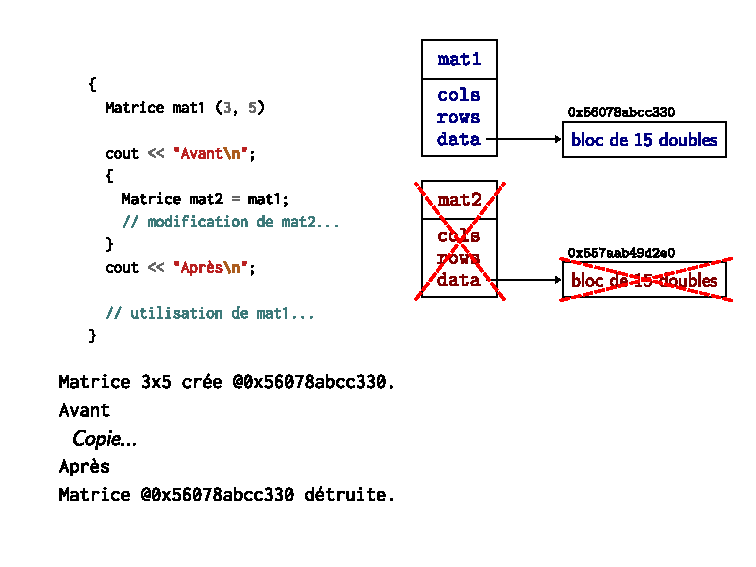
\includegraphics[scale=1]{copiegood2.pdf}
};
\end{tikzpicture}
\end{frame}

%--------------------------------------------------------------------------------------------

\begin{frame}[fragile]{Solution : Constructeur par copie}
  \begin{itemize}
  \item Nécessaire pour effectuer une copie \emph{profonde} (copie contenu mémoire allouée dynamiquement...)
  \item Déclaration :
    \begin{minted}[fontsize=\footnotesize,samepage,mathescape,xrightmargin=0.5cm,xleftmargin=0.5cm]{c++}
      Matrice (const Matrice&);
    \end{minted}
  \item Définition :
    \begin{minted}[fontsize=\footnotesize,samepage,mathescape,xrightmargin=0.5cm,xleftmargin=0.5cm]{c++}
      Matrice::Matrice(const Matrice& other)
        : cols(other.cols), rows(other.rows), data(nullptr)
      {
        data = new double[cols*rows];
        for (unsigned int k = 0; k < cols*rows; k++)
          data[k] = other.data[k];   
      }
    \end{minted}
    \item Utilisation : \texttt{Matrice mat2(mat1);} ou \texttt{Matrice mat2 = mat1;}
    \item Voir exemple dans \texttt{/public/mphyo/M1-C++/TestCopyConstruct}
    \item Alternativement, on peut \emph{interdire la copie} :
    \begin{minted}[fontsize=\footnotesize,samepage,mathescape,xrightmargin=0.5cm,xleftmargin=0.5cm]{c++}
      Matrice (const Matrice&) = delete;
    \end{minted}
  \end{itemize}
\end{frame}

%-----------------------------------------------

\section{Encapsulation}

\begin{frame}[fragile]{Encapsulation : définition}
Encapsulation = interdire/cacher l'accès de certains attributs d'une classe à tout code extérieur à la classe

\begin{itemize}
\item il n'est plus possible d'agir \structure{directement} sur les données d'un objet

\item la modification des attributs de l'objet se fait par \structure{l'intermédiaire de méthodes associées}
\end{itemize}

\structure{Syntaxe :} les mots clés sont \inline{private}, \inline{protected} et \inline{public}
\end{frame}

\begin{frame}[fragile]{Exemple}
\begin{minted}[fontsize=\footnotesize,samepage,mathescape,xrightmargin=0.5cm,xleftmargin=0.5cm]{c++}
class Particule {
private: // facultatif : private par défaut
  // Déclaration des attributs
  double masse_MeV;
  int charge_u;
  ...
};
\end{minted}
\pause
\vspace{1em}
\structure{Conséquence :}
\vspace{1em}
\begin{minted}[fontsize=\footnotesize,samepage,mathescape,xrightmargin=0.5cm,xleftmargin=0.5cm]{c++}
Particule my_kaonplus;
my_kaonplus.masse_MeV = 493.678; // erreur de compilation
\end{minted}
\end{frame}

\begin{frame}[fragile]{Exemple complet (1/2)}
 \begin{minted}[fontsize=\footnotesize,samepage,mathescape,xrightmargin=0.5cm,xleftmargin=0.5cm]{c++}
class Particule {
private:
  // Déclaration des attributs
  double masse_MeV;
  int charge_u;

public:
  // Déclaration des méthodes d'accès
  double get_masse_MeV() const;
  double get_masse_kg() const;
  void set_masse(double masse_MeV_);

  int get_charge_u() const;
  double get_charge_C() const;
  void set_charge(int charge_u_);
};
\end{minted}
\end{frame}

%-----------------------------------------------------------------------

\begin{frame}[fragile]{Exemple complet (2/2)}

\begin{minted}[fontsize=\footnotesize,samepage,mathescape,xrightmargin=0.5cm,xleftmargin=0.5cm]{c++}
// Définition des méthodes
double Particule::get_masse_MeV() const {
  return masse_MeV;
}

void Particule::set_masse(double masse_MeV_) {
  if (masse_MeV_ > 0)
    throw std::range_error("Masse de particule négative !");
  masse_MeV = masse_MeV_;
}

void Particule::set_charge(int charge_u_) {
  if (charge_u_ > 1 or charge_u_ < -1)
    throw std::range_error("Charge de particule doit être -1, 0, ou 1");
  charge_u = charge_u_;
}
...
\end{minted}
\pause
\begin{minted}[fontsize=\footnotesize,samepage,mathescape,xrightmargin=0.5cm,xleftmargin=0.5cm]{c++}
Particule my_kaonplus;
my_kaonplus.set_charge(+1);
double masse = my_kaonplus.get_masse_MeV();
\end{minted}

\end{frame}

%----------------------------------------------------------------------

\begin{frame}[fragile]{Exemple (incomplet) : \texttt{Matrice}}

Il faut interdire l'accès de \texttt{data} à l'utilisateur.
\vspace{1em}
\begin{minted}[fontsize=\footnotesize,samepage,mathescape,xrightmargin=0.5cm,xleftmargin=0.5cm]{c++}
class Matrice {
public:
  ...
  double& accès(int row, int col);  // Accès à un élément de la matrice

private:
  double* data;
  unsigned int cols, rows;
};
\end{minted}
\pause
\vspace{1em}
\begin{minted}[fontsize=\footnotesize,samepage,mathescape,xrightmargin=0.5cm,xleftmargin=0.5cm]{c++}
double& Matrice::accès(int row, int col) {
  if (row < 0 or row >= rows or col < 0 or col >= cols)
    throw std::out_of_range();
  return data[ row*cols + col ]; // renvoie une référence
}
\end{minted}
\pause
\vspace{1em}
\begin{minted}[fontsize=\footnotesize,samepage,mathescape,xrightmargin=0.5cm,xleftmargin=0.5cm]{c++}
mat1.accès(1, 2) = 4.2;  // modification via référence
\end{minted}

\end{frame}

%---------------------------------------------------------------------

\begin{frame}[fragile]{Intérêts de l'encapsulation}
\begin{itemize}
\item Lors de la programmation et surtout de la réutilisation d'un objet dans un
autre programme, l'encapsulation empêche la modification non voulue des données
membres

\item L'objet, vu de l'extérieur, \structure{n'est caractérisé que par son \emph{interface}\footnote{c'est à dire l'ensemble des attributs et méthodes effectivement utiles pour l'utilisateur}}\pause :

\begin{enumerate}[<+->]
\item pas d'ambiguïté pour l'utilisateur (\textit{ait-je le droit de modifier cet attribut ?} \textit{est-ce que faire ceci peut faire planter le programme ?}); plus simple; moins d'erreurs
\item la maintenance et l'amélioration de l'objet sont grandement facilitées; tant que la finalité des méthodes et attributs de l'interface publique ne change pas, on peut modifier les rouages sans perturber pour autant les utilisateurs de la classe
\item la classe est facilement réutilisable (cf. héritage)
\end{enumerate}
\end{itemize}
\end{frame}

%----------------------------------------------------

\begin{frame}[fragile]{Intérêts de l'encapsulation}

Règle assez générale :
\begin{itemize}[<+->]
\item \inline{private} si l'attribut doit être protégé
\item Si on envisage qu'un attribut puisse être contraint dans le futur\footnote{en particulier dans une classe fille, cf. cours sur l'héritage} $\rightarrow$ \inline{private}/\inline{protected}
\item Sinon, on \emph{peut} laisser \inline{public}, en particulier si cela évite une lourdeur syntaxique (setters \& getters, ex. : \texttt{vec3}, \texttt{point}...)
\item Dans le doute, préférer \inline{private}/\inline{protected}
\end{itemize}

\end{frame}

\end{document}
